\documentclass[tikz,border=3mm]{standalone}
\usetikzlibrary{arrows.meta,calc}
\begin{document}
\pagecolor{white}
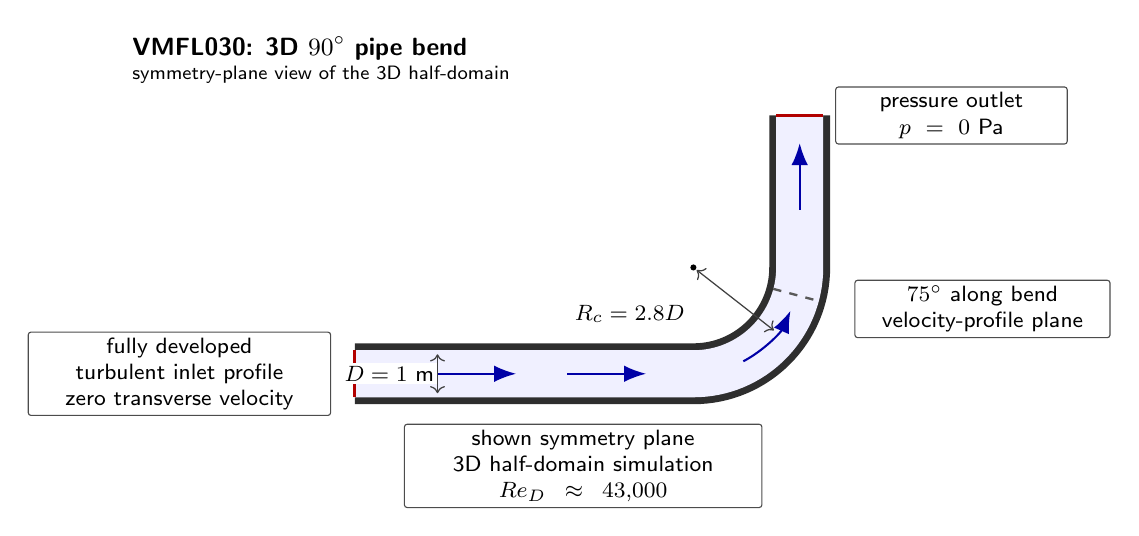
\begin{tikzpicture}[
  font=\sffamily\footnotesize,
  flow/.style={-{Latex[length=2.8mm]}, line width=0.75pt, draw=blue!65!black},
  dim/.style={<->, line width=0.45pt, draw=black!75, shorten <=1.5pt, shorten >=1.5pt},
  section/.style={draw=red!70!black, line width=1.1pt},
  profile/.style={draw=black!65, dashed, line width=0.85pt},
  bc/.style={draw=black!70, fill=white, rounded corners=1pt, inner sep=2pt, align=center}
]

\node[font=\sffamily\bfseries\small, anchor=west] at (0.10,4.90)
  {VMFL030: 3D $90^\circ$ pipe bend};
\node[font=\sffamily\scriptsize, anchor=west] at (0.10,4.57)
  {symmetry-plane view of the 3D half-domain};

\def\r{1.35}
\def\xc{7.35}
\def\yc{2.12}
\def\w{0.30}
\def\xin{3.05}
\def\yin{\yc-\r}
\def\xout{\xc+\r}
\def\yout{4.05}

\draw[black!82, line width=22pt, line cap=butt, line join=round]
  (\xin,\yin) -- (\xc,\yin) arc[start angle=-90,end angle=0,radius=\r] -- (\xout,\yout);
\draw[blue!6, line width=17pt, line cap=butt, line join=round]
  (\xin,\yin) -- (\xc,\yin) arc[start angle=-90,end angle=0,radius=\r] -- (\xout,\yout);

% Boundary planes and labels.
\draw[section] (\xin,\yin-\w) -- (\xin,\yin+\w);
\draw[section] (\xout-\w,\yout) -- (\xout+\w,\yout);
\node[bc, anchor=east, text width=37mm] at (\xin-0.30,\yin)
  {fully developed\\turbulent inlet profile\\zero transverse velocity};
\node[bc, anchor=west, text width=28mm] at (\xout+0.45,\yout)
  {pressure outlet\\$p=0$ Pa};

% Flow direction.
\draw[flow] (3.80,\yin) -- (5.10,\yin);
\draw[flow] (5.75,\yin) -- (6.75,\yin);
\draw[flow] ({\xc+\r*cos(-62)},{\yc+\r*sin(-62)}) arc[start angle=-62,end angle=-24,radius=\r];
\draw[flow] (\xout,2.85) -- (\xout,3.70);

% Bend radius and diameter.
\coordinate (bendcenter) at (\xc,\yc);
\coordinate (radiuspoint) at ({\xc+\r*cos(-38)},{\yc+\r*sin(-38)});
\draw[dim] (bendcenter) -- (radiuspoint);
\node[fill=white, inner sep=1pt, anchor=east] at (7.28,1.53)
  {$R_c=2.8D$};
\fill[black] (bendcenter) circle (1.1pt);

\draw[dim] (4.10,\yin-\w) -- node[left, fill=white, inner sep=1pt]
  {$D=1$ m} (4.10,\yin+\w);

% 75 degree velocity-profile plane.
\coordinate (profileInner) at ({\xc+(\r-\w)*cos(-15)},{\yc+(\r-\w)*sin(-15)});
\coordinate (profileOuter) at ({\xc+(\r+\w)*cos(-15)},{\yc+(\r+\w)*sin(-15)});
\draw[profile] (profileInner) -- (profileOuter);
\node[bc, anchor=west, text width=31mm] at ($(profileOuter)+(0.45,-0.10)$)
  {$75^\circ$ along bend\\velocity-profile plane};

\node[bc, text width=44mm] at (5.95,-0.40)
  {shown symmetry plane\\3D half-domain simulation\\$Re_D\approx43{,}000$};

\end{tikzpicture}
\end{document}
